\chapter{Information Visualization}

\label{chap:InfoVis}

Information visualization is the science of representing abstract information as interactive graphics to present and analyze it more efficiently. These two goals of presenting and analyzing abstract information in a visual form are built on the properties of human visual perception, which include the rapid scanning, recognition and recollection of visual information as well as the automatic detection of patterns in it. In contrast to textual representations of data, the processing of well-designed visualizations requires much less cognitive effort because it leverages features of the human visual processing system such as preattentive processing, meaning that certain visual attributes can be processed very quickly and without any conscious effort \parencite{PreattentiveProcessing}. 

In addition to visuals being easier to assimilate by humans, a purely textual and statistical view on data can also lead to erroneous assumptions as demonstrated by \cite{AnscombesQuartet} in the infamous visualization of four completely different datasets that have identical summary statistics, called Anscombe's Quartet. An observer trying to understand these sets of data purely from their statistics would mistakenly deem them to be identical because their inequality will only become obvious after carefully examining and comparing the individual entries in the datasets themselves, which is a tedious and error-prone task when not aided by visual representations like Figure \ref{fig:AnscombesQuartet}. Even though Anscombe's Quartet is very likely the most famous example to demonstrate this characteristic, it is certainly not the only set of datasets that possesses it, as has been shown by \cite{GenDataIdenticalStatisticsDissimilarGraphics}.

\begin{figure}[tp]
    \centering
    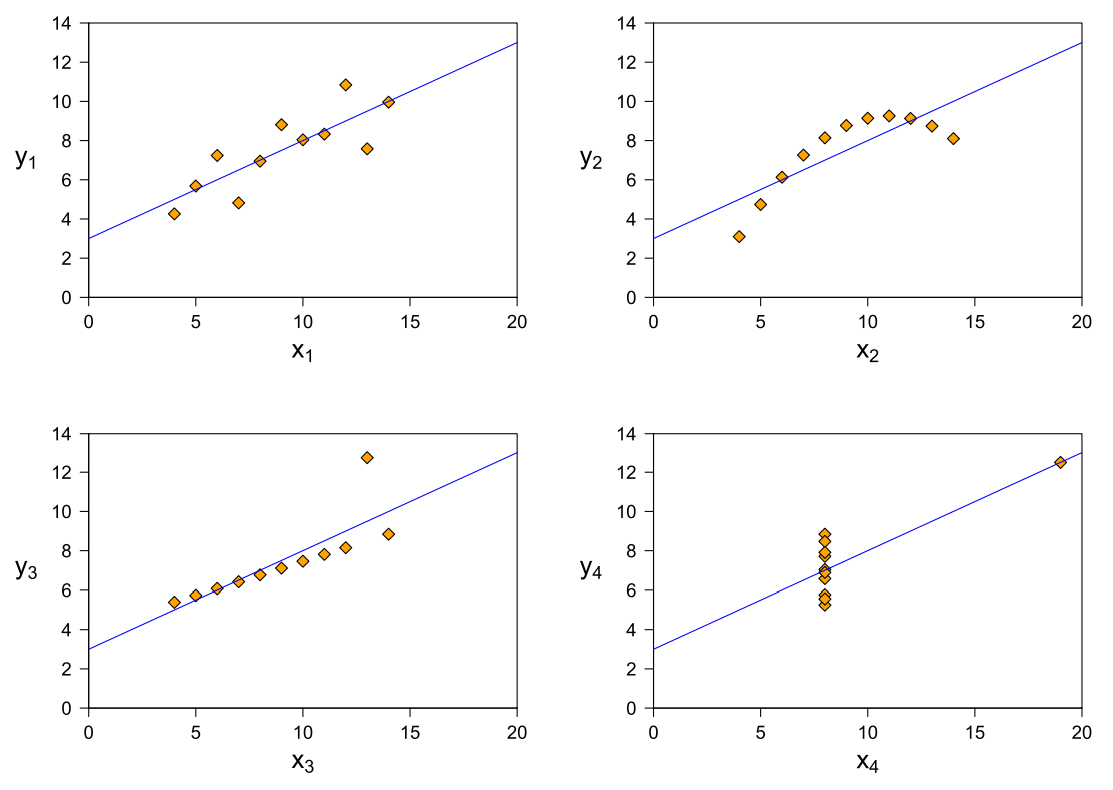
\includegraphics[keepaspectratio,width=\linewidth,height=\fullh / 3]
    {images/anscombes-quartet.png}

    \caption[Anscombe's Quartet]{
        Anscombe's Quartet consists of four distinct sets of data that share identical summary statistics. The difference between these datasets is only obvious by carefully examining the textual data or by plotting it. \imgcredit{Image extracted from \cite{IVISCourseNotes} with kind permission by Keith Andrews. \TODO{Get SVG PDF version from Keith}}
    }
    \label{fig:AnscombesQuartet}
\end{figure}

Regarding terminology, this work adheres to the separation of the field of visualization into three main subfields as described by \cite{IVISCourseNotes}.

\begin{enumerate}
    \item Information Visualization: Deals with abstract data, which has no inherent presentation and for which a suitable type of visualization has to be chosen.
    \item Geographic Visualization: Deals with map-based data that has an inherent spatial dimension. 
    \item Scientific Visualization: Deals with object-related data that has inherent presentation, which is usually related to the object's real world representation.
\end{enumerate}

In addition to these three subfields, \cite{IVISCourseNotes} defines the often used term Data Visualization as the intersection of Geographic Visualization and Information Visualization. Therefore, it deals with visualizing spatial as well as abstract data.

Visualizations presented in an interactive medium do not merely consist of visual representations. In order to analyze more complex datasets, it is equally important to provide means for interacting with these representations because without interaction, a visualization becomes a static image, which has only very limited usefulness when dealing with large and multidimensional data. Even though the majority of the attention in the field of Information Visualization has been put on the presentational aspect of visualizations, a lot of research has also been conducted on their interactive aspects. Many taxonomies have been formulated with the goal of defining the design space of interactions to support analytic reasoning, but they vary greatly depending on the concepts they are focusing on. Some taxonomies have been defined on the concept of low-level interaction techniques \parencite{TheEyesHaveIt,GrammarOfGraphics}, providing a very system-centric view on interaction, while other taxonomies focus on user tasks \parencite{LowLevelComponentsOfAnalyticActivity} without them being tightly bound to interacting with visualizations. \cite{RoleOfInteractionInInformationVisualization} aims to provide a view that is in between the purely system-centric and purely user-centric extremes by defining a taxonomy based on user intent. The categories of this taxonomy are listed in Table \ref{tab:UserIntentCategories}, and they form a good framework with which interactivity in the context of Information Visualization can be discussed. 

\begin{table}[tp]
    \centering
    \begin{tabularx}{\linewidth}{| l | X | X |}
        \hline
        \textbf{Category} & \textbf{Description} & \textbf{Examples} \\ \hline
        Select & Mark items as interesting. &  \\ \hline
        Explore & Show different items. & Panning, direct-walk  \\ \hline
        Reconfigure & Show a different arrangement. & Dimension configuration, position adjustments \\ \hline
        Encode & Show a different representation. & Change chart type, orientation, colors, shapes, ... \\ \hline
        Abstract/Elaborate & Show more or less detail. & Details-on-demand (drill-down, sunburst, tooltips, zooming)  \\ \hline
        Filter & Show items based on conditions. & Dynamic query controls   \\ \hline
        Connect & Show related items. & Highlight connected items, highlight item in different representations   \\ \hline
        
    \end{tabularx}
    \caption[Categories of Interaction Based on User Intent]
    {
        This table shows the different categories of interacting with visualizations based on user intent.
        \imgcredit{Table adapted from \cite{RoleOfInteractionInInformationVisualization}}
    }
    \label{tab:UserIntentCategories}
\end{table}

\section{History of Information Visualization}

The history of Information Visualization goes back a long time with one of the earliest examples dating back to the 10th century, when an unknown astronomer created a chart about the movement of the most prominent planets \parencite{CommentariiInSomniumScipionis}, shown in Figure \ref{fig:PlanetaryMovements}. Other noteworthy early visualizations include the first occurrence of the principle \cite{VisualDisplayOfQuantitativeInformation} later coined "small multiples" in a 1626 chart demonstrating sunspot changes (Figure \ref{fig:SunspotChanges}) by \cite{RosaUrsina} and a 1644 chart displaying longitudinal distance determinations between Toledo and Rome (Figure \ref{fig:RomeToledoLongitude}) by Michael Florent van Langren. 

\begin{figure}[tp]
    \centering
    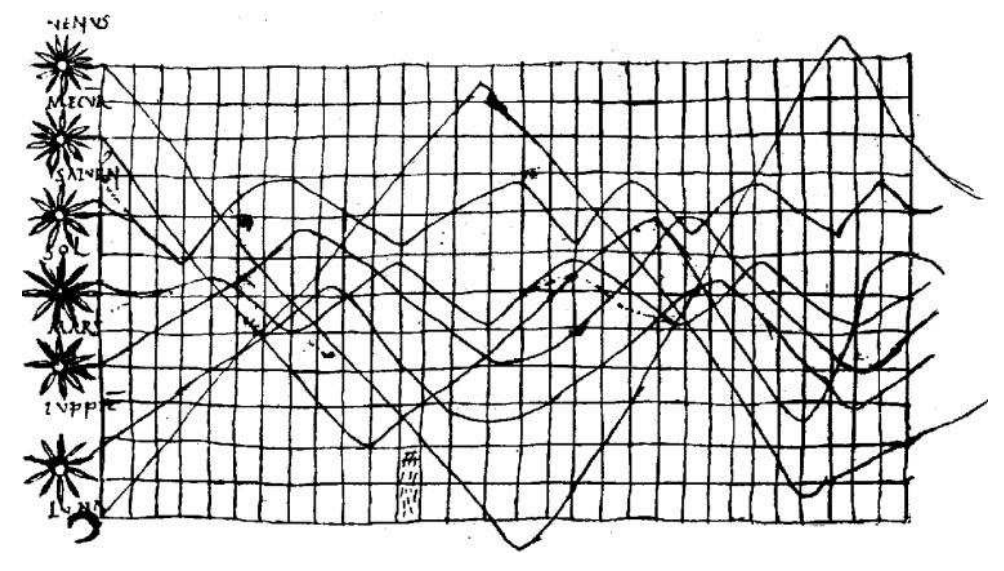
\includegraphics[keepaspectratio,width=\linewidth,height=\fullh / 3]
    {images/planetary-movements.png}
    \caption[Chart of Planetary Movements from the Tenth Century]{
        A chart created by an unknown astronomer in the tenth century depicting the movements of the seven most prominent planets. \imgcredit{Image extracted from \cite{BriefHistoryOfDataVis}. Original appearance in \cite{CommentariiInSomniumScipionis}.}
    }
    \label{fig:PlanetaryMovements}
\end{figure}

\begin{figure}[tp]
    \centering
    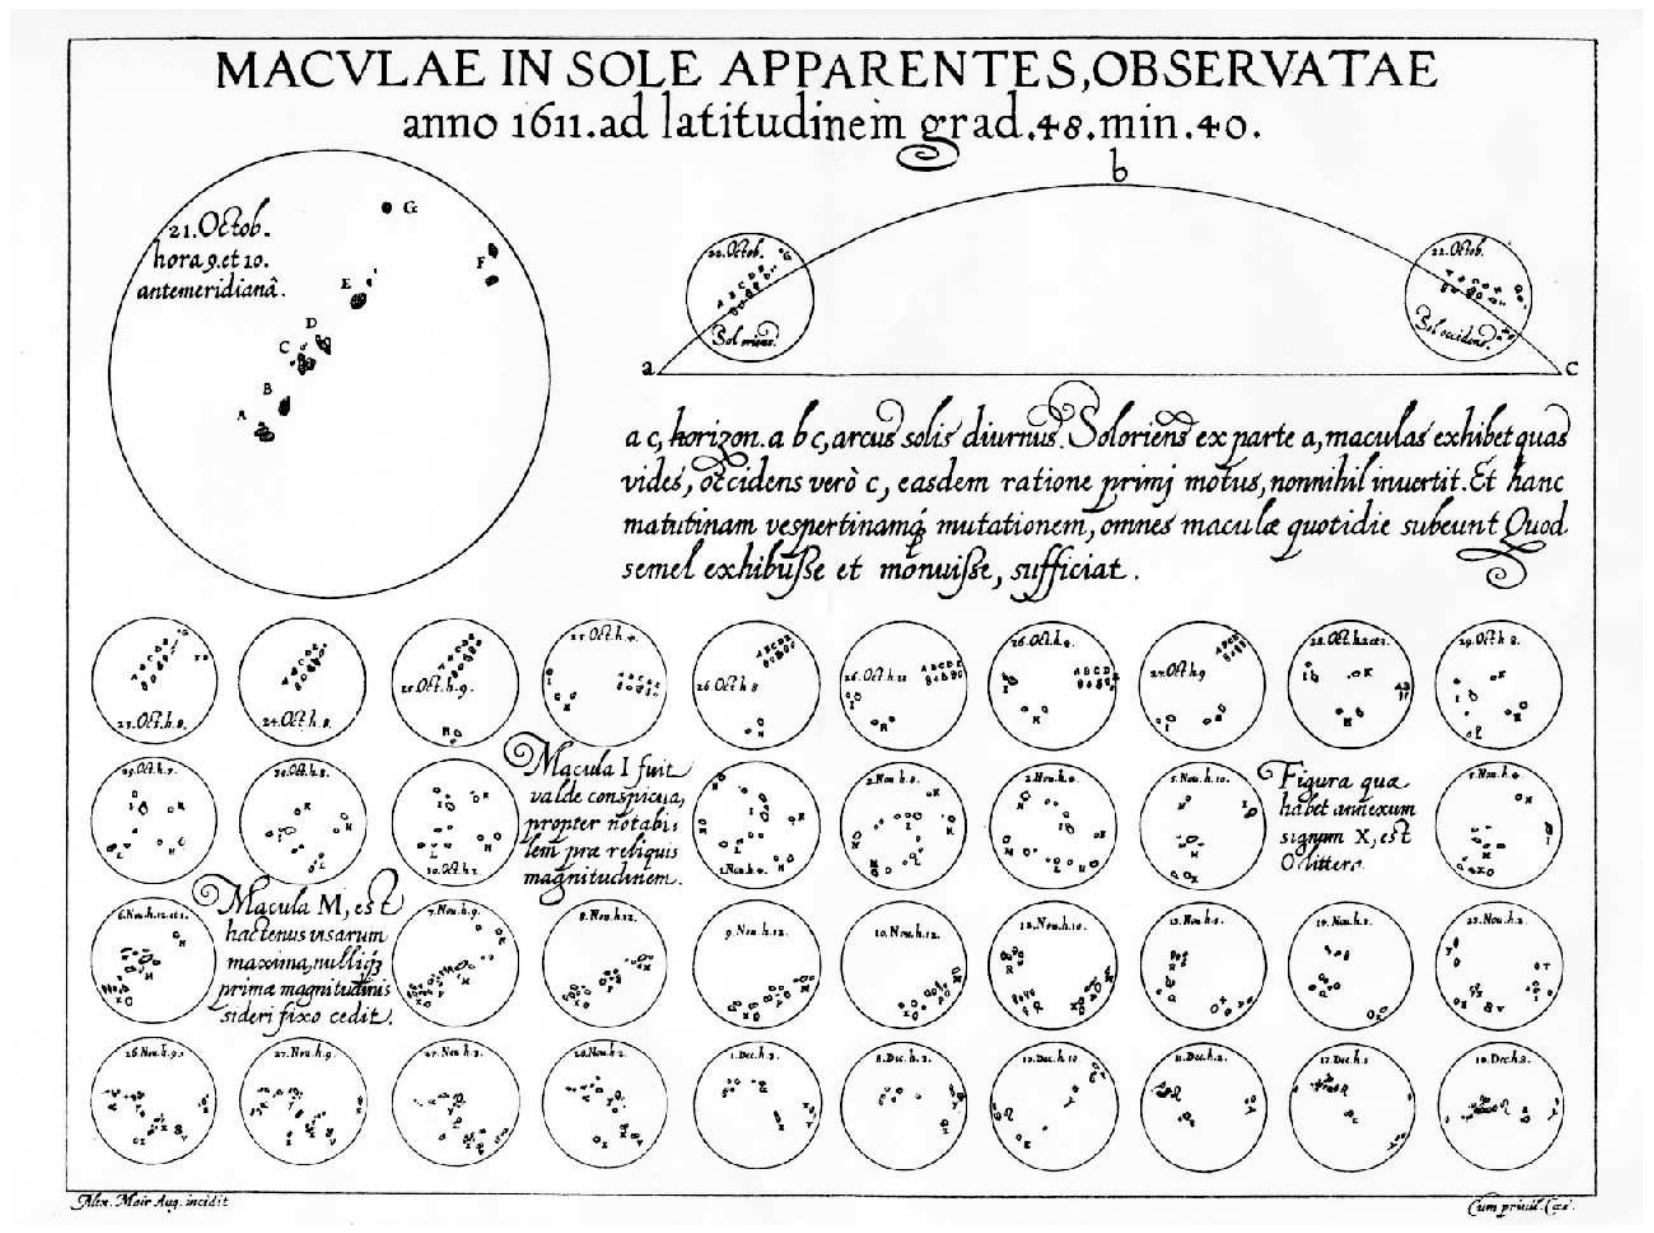
\includegraphics[keepaspectratio,width=\linewidth,height=\fullh / 3]
    {images/sunspot-changes.png}
    \caption[Chart of Changes in Sunspots from 1626]{
        This chart shows the observed changes in sunspots based on recordings of two months of data from 1611. It is the first occurrence of the principle later called "small multiples" by \cite{VisualDisplayOfQuantitativeInformation}. \imgcredit{Image extracted from \cite{BriefHistoryOfDataVis}. Original appearance in \cite{RosaUrsina}.}
    }
    \label{fig:SunspotChanges}
\end{figure}

\begin{figure}[tp]
    \centering
    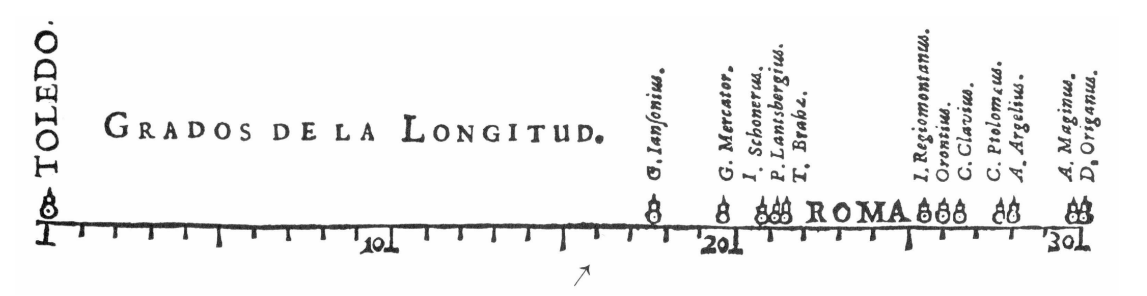
\includegraphics[keepaspectratio,width=\linewidth,height=\fullh / 3]
    {images/rome-toledo-longitude.png}
    \caption[Chart of Longitudinal Distance Determinations Between Toledo and Rome From 1644]{
        This chart compares the twelve known estimates in longitudinal distance between Rome and Toledo by various astronomers. The correct distance is marked by the arrow beneath. It is considered to be the first visual representation of statistical data. \imgcredit{Image extracted from \cite{BriefHistoryOfDataVis}. Original appearance in \cite{VisualExplanations}.}
    }
    \label{fig:RomeToledoLongitude}
\end{figure}

William Playfair (1759 - 1823) is by many considered to be one of the forefathers of modern visualizations because his published works contain the first occurrences of many graphical forms that are still widely used today. In one of his earlier works \parencite{CommercialAndPoliticalAtlas} he introduced the concepts of line (Figure \ref{fig:PlayfairLineChart}), bar (Figure \ref{fig:PlayfairBarChart}) and area charts (Figure \ref{fig:PlayfairAreaChart}) to communicate economic factors of England during the eighteenth century. In a related later work \parencite{StatisticalBreviary} he uses the first ever published pie and circle charts to show and compare the resources of states and kingdoms in Europe. The charts he created are very similar to modern ones because they already contain all the major elements found in today's visualizations, such as labeled axes, grids, titles and color-based categorization.

\begin{figure}[tp]
    \centering
    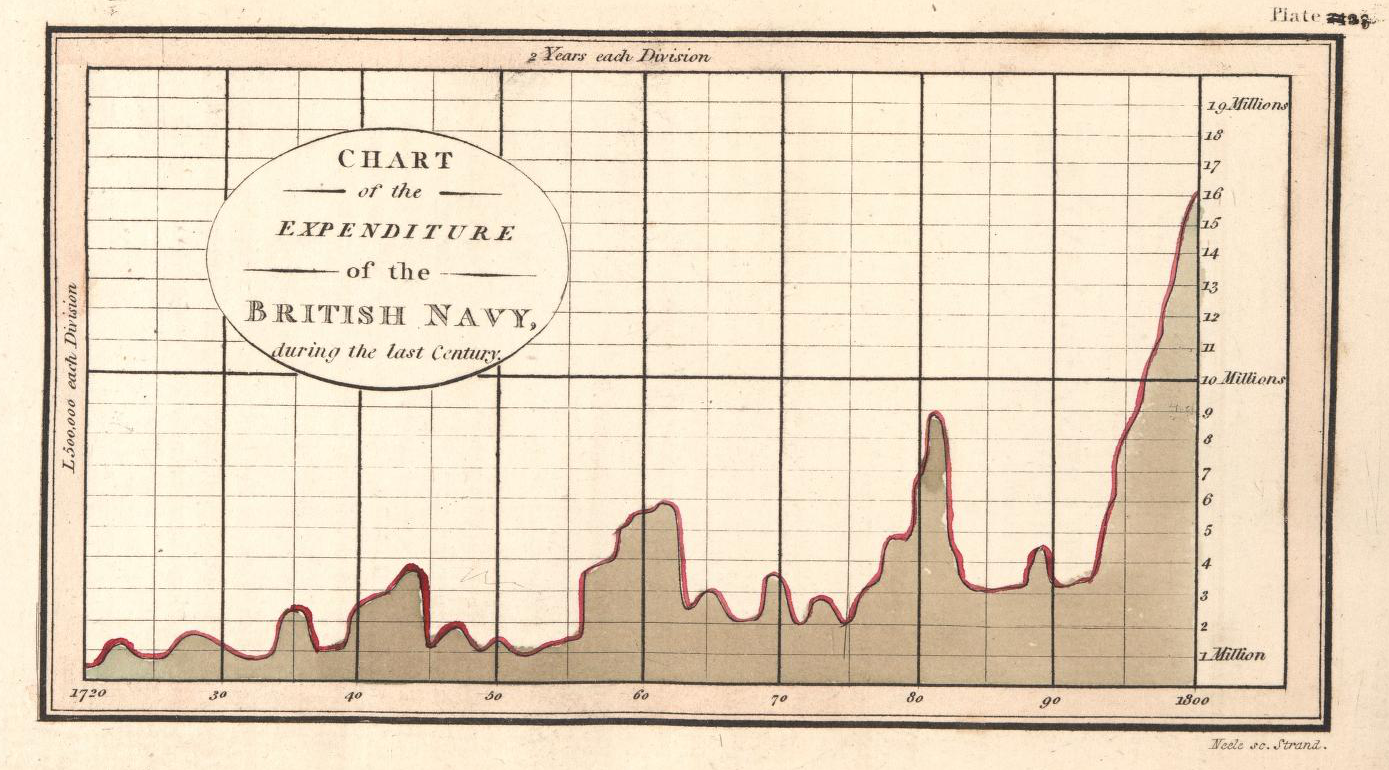
\includegraphics[keepaspectratio,width=\linewidth,height=\fullh / 3]
    {images/playfair-line-chart.png}
    \caption[Line Chart by William Playfair From 1786]{
        This chart shows the expenditure of the British navy during the eighteenth century as a line chart. It was published in 1786 and is considered to be one of the first occurrences of a line chart that contains all components found in modern visualizations. \imgcredit{Image extracted from Schoenberg Center for Electronic Text and Image (SCETI). Used under the terms of Creative Commons CC BY 2.5.}
    }
    \label{fig:PlayfairLineChart}
\end{figure}

\begin{figure}[tp]
    \centering
    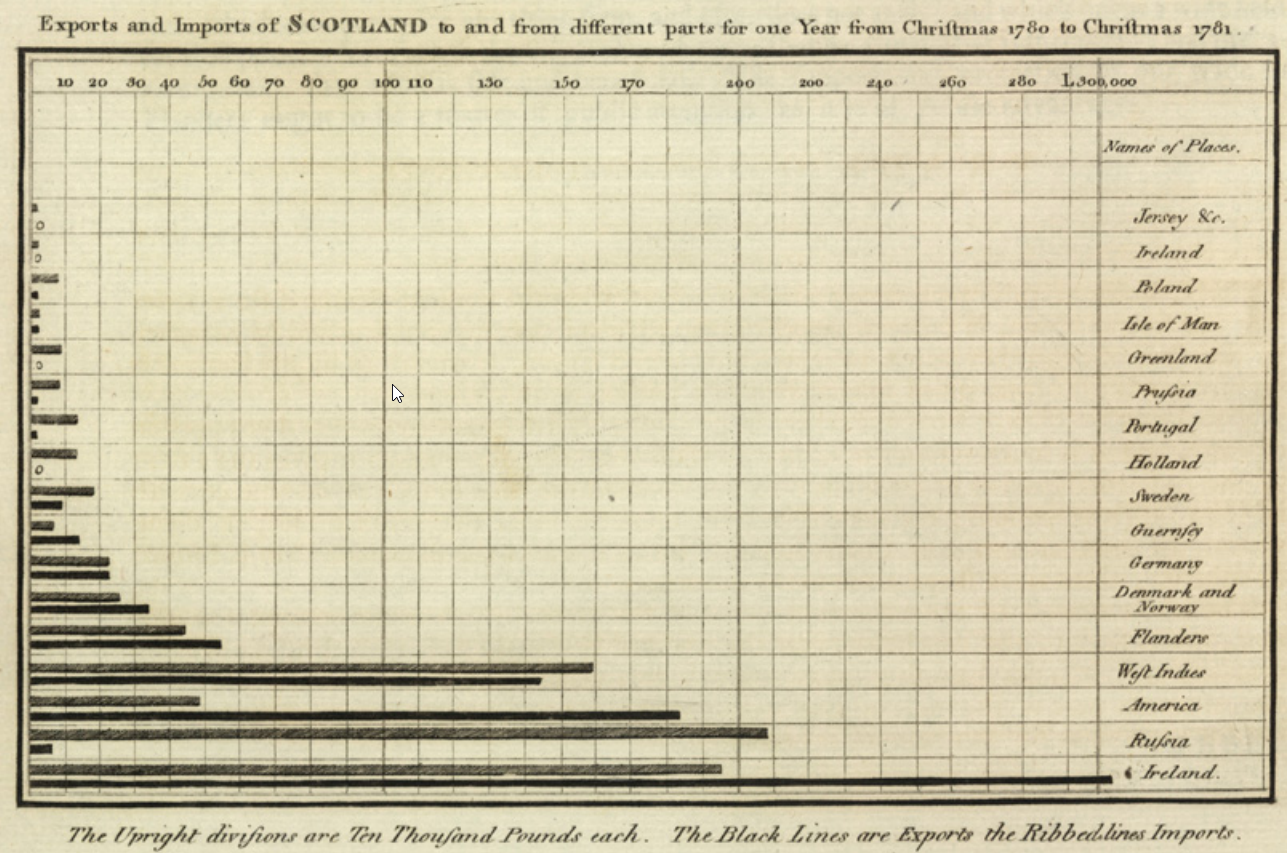
\includegraphics[keepaspectratio,width=\linewidth,height=\fullh / 3]
    {images/playfair-bar-chart.png}
    \caption[Bar Chart by William Playfair from 1786]{
        This chart shows England's exports and imports from and to Scotland in 1781 visualized as a bar chart. It was published in 1786 and is considered to be one of the first occurrences of a bar chart that contains all components found in modern visualizations. \imgcredit{Image extracted from Schoenberg Center for Electronic Text and Image (SCETI). Used under the terms of Creative Commons CC BY 2.5.}
    }
    \label{fig:PlayfairBarChart}
\end{figure}

\begin{figure}[tp]
    \centering
    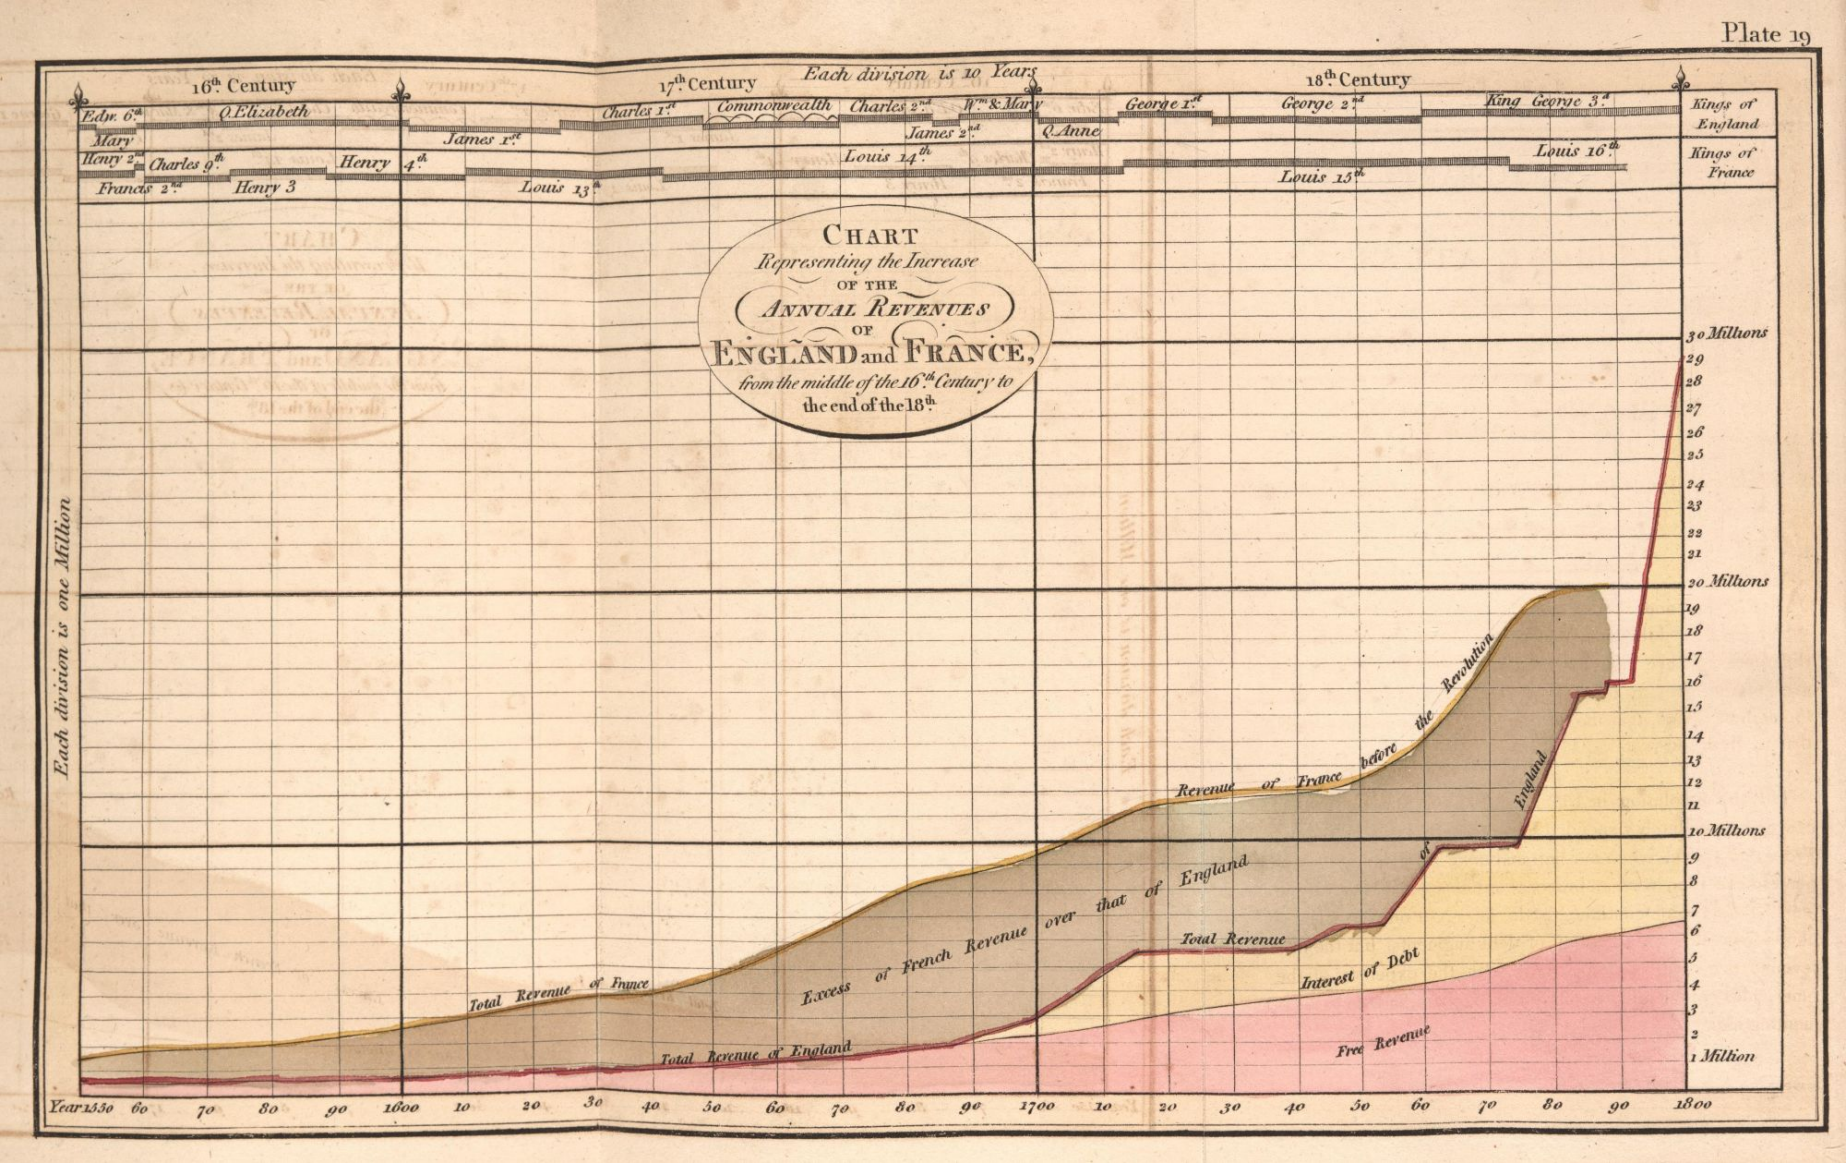
\includegraphics[keepaspectratio,width=\linewidth,height=\fullh / 3]
    {images/playfair-area-chart.png}
    \caption[Area Chart by William Playfair from 1786]{
        This chart shows the annual revenues of England and France between 1550 and 1800 visualized as an area chart. It was published in 1786 and is considered to be one of the first occurrences of an area chart that contains all components found in modern visualizations. \imgcredit{Image extracted from Schoenberg Center for Electronic Text and Image (SCETI). Used under the terms of Creative Commons CC BY 2.5.}
    }
    \label{fig:PlayfairAreaChart}
\end{figure}

Albeit not directly an information visualization but rather a geographic one, the dot map created by \cite{ModeOfCommunicationOfCholera} in 1855 to trace cholera outbreaks in London (Figure \ref{fig:CholeraDotMap}) is undoubtedly one of the most famous and influential visualizations in history. It was used to identify a cluster of cholera-related deaths near a contaminated water pump on Broad Street, leading to the recognition of cholera as a waterborne disease.

\begin{figure}[tp]
    \centering
    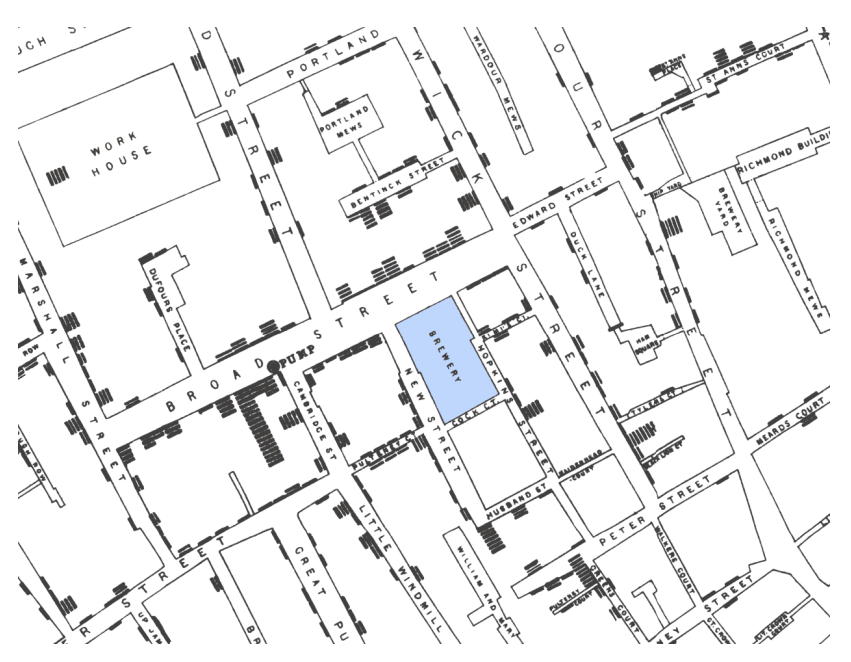
\includegraphics[keepaspectratio,width=\linewidth,height=\fullh / 3]
    {images/cholera-dot-map.png}
    \caption[Dot Map Plotting Cholera Deaths in London From 1855]{
        This iconic chart was created by Dr. John Snow in 1855 to identify a clustering of cholera-related deaths near Broad Street in London. It was used to identify a contaminated water pump and to illustrate the waterborne nature of the disease. The data being map-based, this chart is an example of a data visualization rather than an information visualization. \imgcredit{Image extracted from \cite{IVISCourseNotes}. Original appearance in \cite{ModeOfCommunicationOfCholera}.}
    }
    \label{fig:CholeraDotMap}
\end{figure}

It would go amiss not to mention Florence Nightingale (1820 - 1910) when talking about the history of information visualization. She was a British statistician, social reformer, founder of modern nursing and might be the first person who used visualizations to persuade others of a need for change. During her service as a superintendent of nurses in the Crimean War, she realized that a large share of deaths in hospitals resulted from preventable diseases that originated in poor sanitary conditions. One of her contributions to the field of information visualization was the creation of a new type of diagram, called a rose or polar-area chart. These charts were used to communicate the data she collected on the mortality of soldiers during the war and to grab the attention of politicians and the public. One of those charts can be seen in Figure \ref{fig:NightingalePolarAreaChart}. \TODO{Cite Nightingale paper}

\begin{figure}[tp]
    \centering
    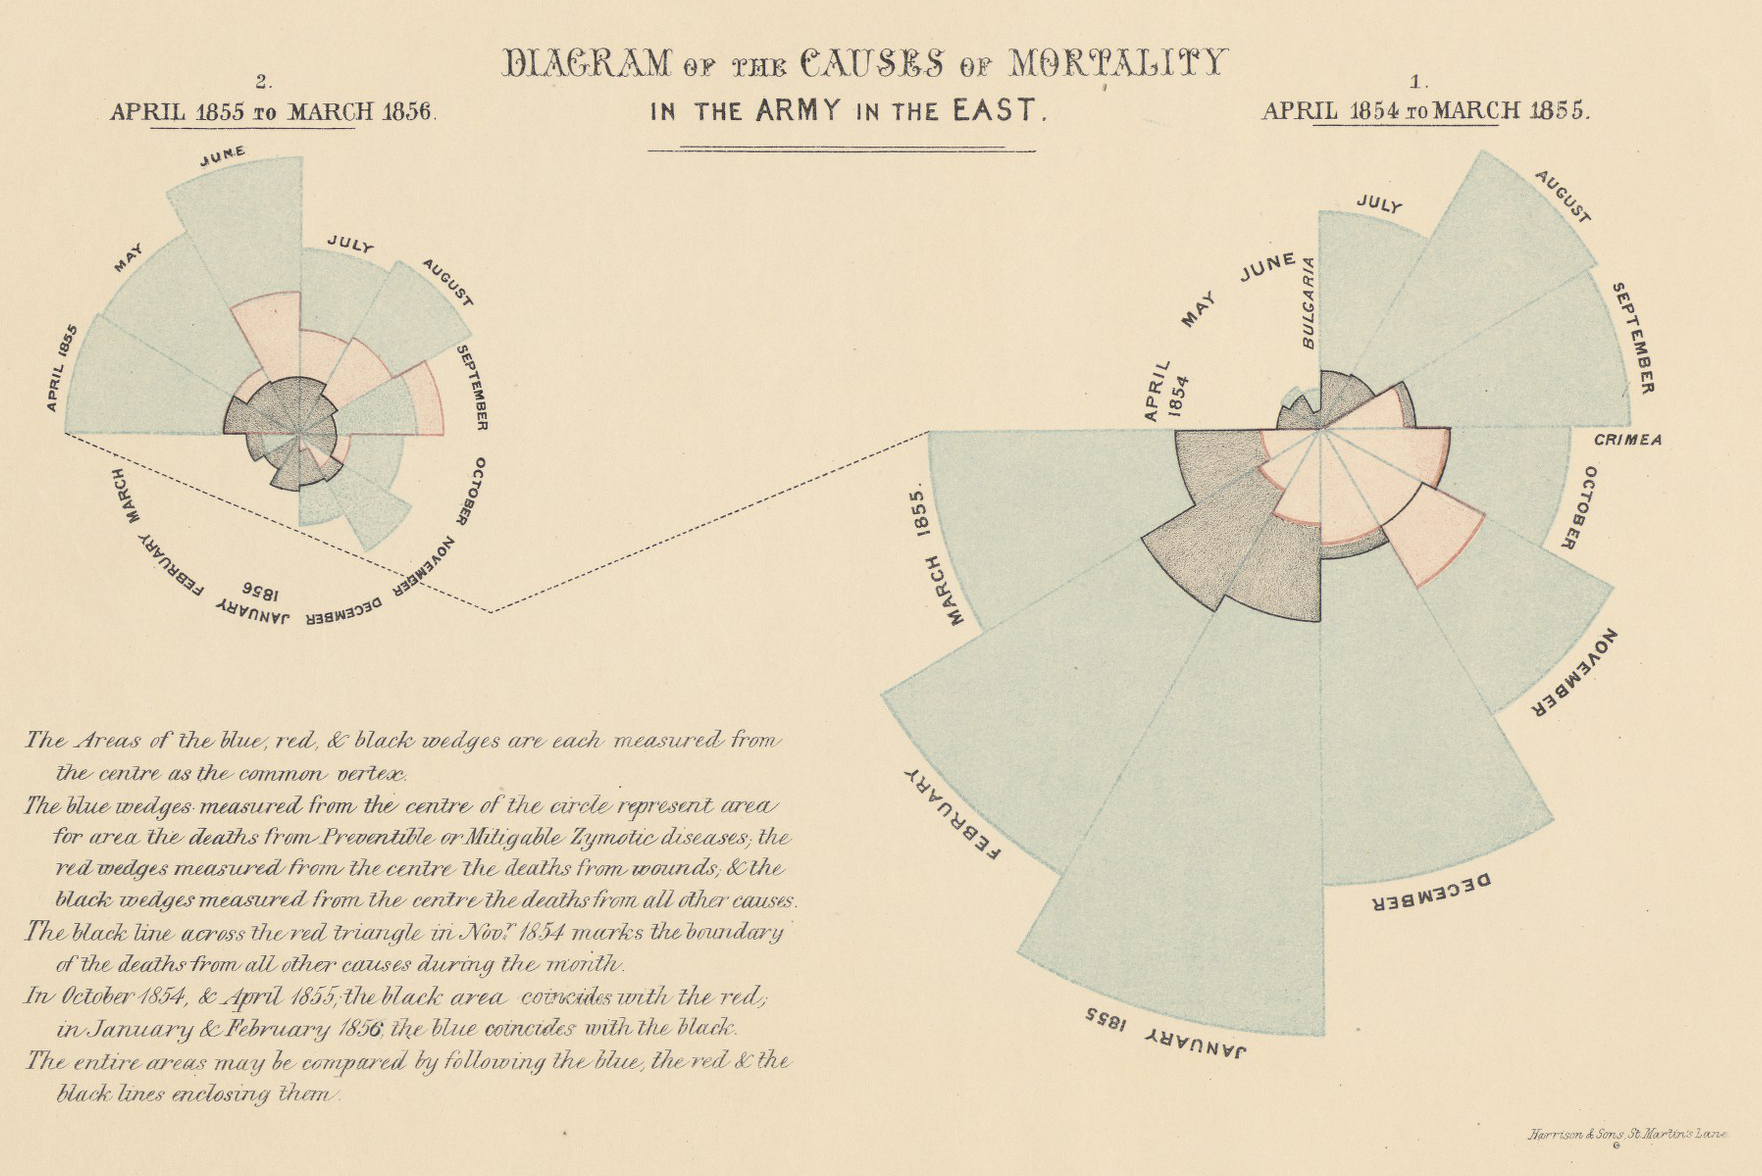
\includegraphics[keepaspectratio,width=\linewidth,height=\fullh / 3]
    {images/nightingale.png}
    \caption[Polar-Area Chart by Florence Nightingale From 1859]{
        This is one of the polar-area charts that Florence Nightingale created in 1859 to convince others of a need for more sanitary conditions in hospitals. It visualizes the causes of mortality for soldiers during the Crimean War and demonstrates that a large percentage of patients died from preventable diseases that are linked to unsanitary environments.
        \imgcredit{Image extracted from Harvard Library. Used under the terms of Creative Commons Attribution 4.0.}
    }
    \label{fig:NightingalePolarAreaChart}
\end{figure}

Modern visualizations benefit from the interactive nature of the devices used to consume them. They are allowed to be a lot more complex than static visualizations because various interaction techniques enable users to navigate large amounts of data and make sense of it. High-D by the company Macrofocus \parencite{HighD} has been chosen as a representative example of such a visual analytics tool and a screenshot of its interface during the analysis of a sample dataset can be seen in Figure \ref{fig:HighD}.

\begin{figure}[tp]
    \centering
    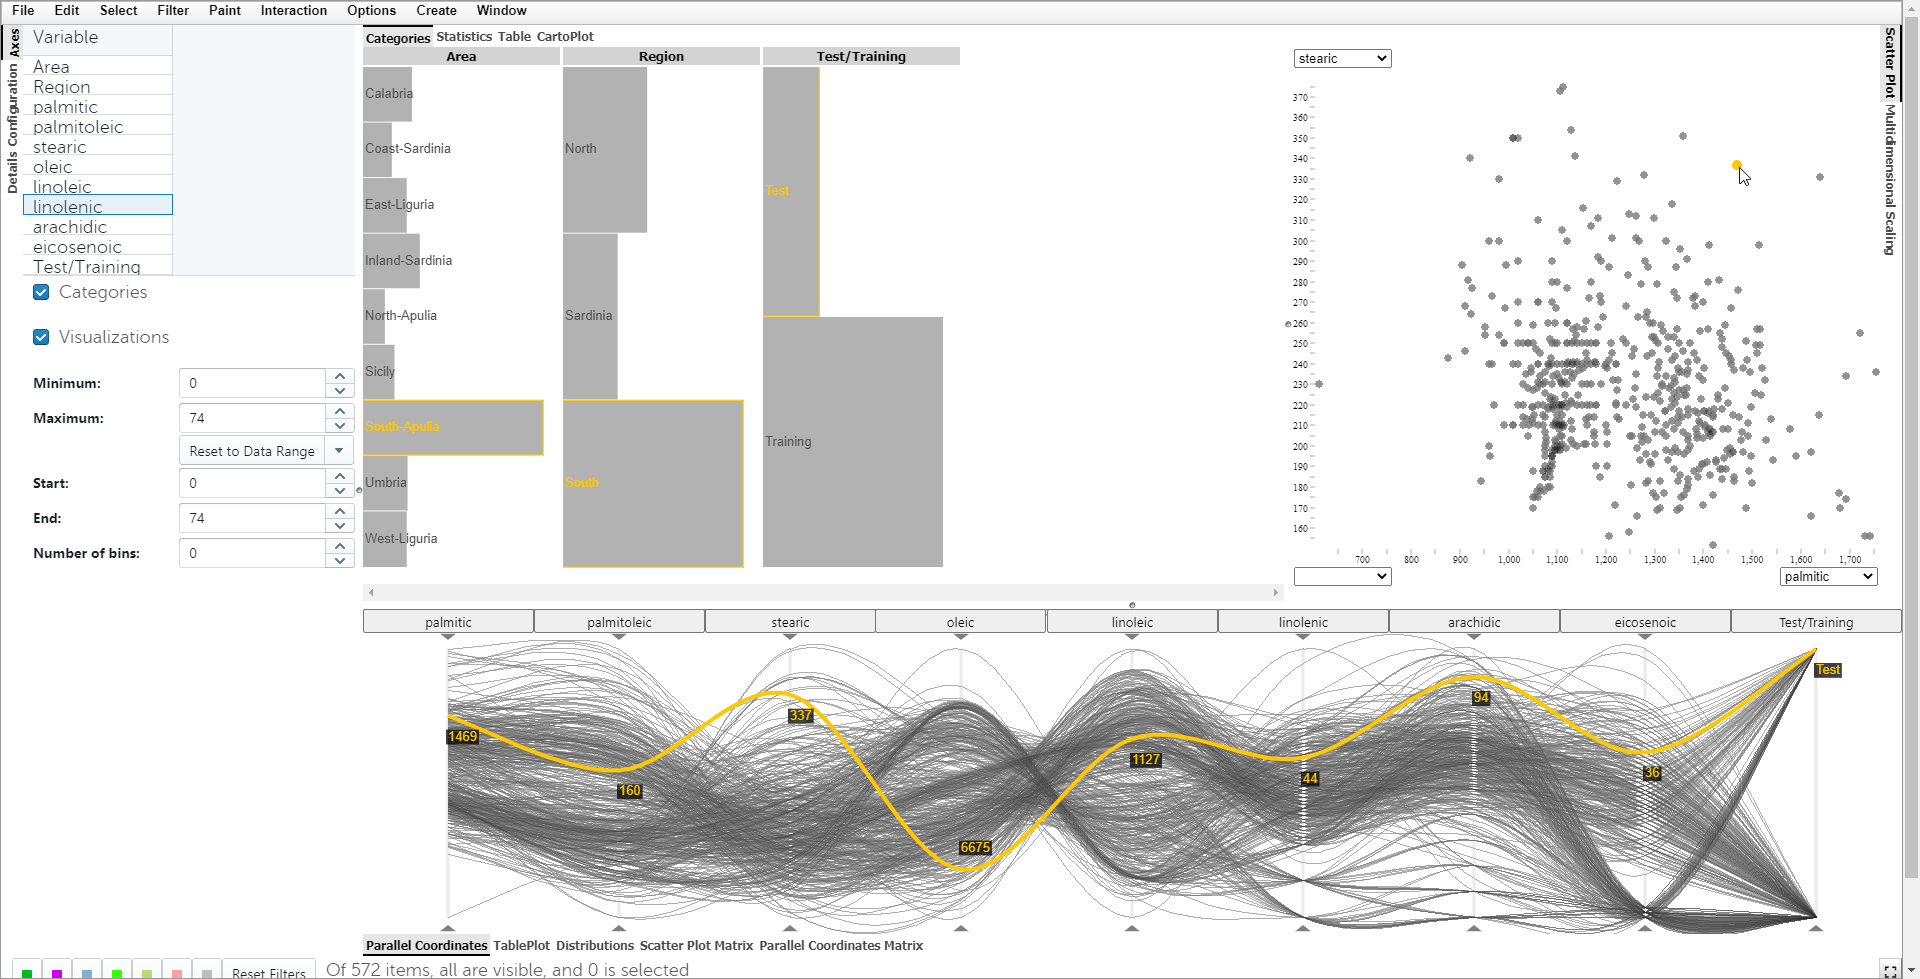
\includegraphics[keepaspectratio,width=\linewidth,height=\fullh / 3]
    {images/high-d.png}
    \caption[Screenshot of High-D]{
        High-D from the company Macrofocus is a visual analytics tool that is specialized in analyzing multidimensional data. 
        \imgcredit{Screenshot of \cite{HighD} taken by the author of this work.}
    }
    \label{fig:HighD}
\end{figure}

It is out of the scope of this work to provide a detailed account over the long and eventful history of information visualization and this section only provides a brief and very selective view on the topic. Much more comprehensive works exist that go significantly deeper into details of the various actors and the intricate influences they had on each other. Recommendable sources for further reading on the history of visualization include \cite{BriefHistoryOfDataVis}, \cite{HistoryOfDataVisAndGraphicCommunication} and \cite{HistoryOfInformationGraphics}.

\section{Responsive Web Design}
\label{sec:RWD}

Influenced by the increasing use of mobile devices and their vastly varying screen sizes, responsive web design has established itself as the predominant way of designing web pages. The core idea of responsive web design is that instead of designing pages for different types of devices, website authors create a single design for a page that adapts to the characteristics of the consuming device. The term "Responsive Web Design" has been defined by \cite{ResponsiveWebDesign} where the author differentiates between flexible and responsive web designs. It states that a flexible web design, which merely fluidly scales blocks of content to make them fit into the width of a browser window, is not enough to provide a good experience for users. Such designs will work well enough for similarly sized viewports to the one they were created for, but they will lead to noticeable artifacts on lower resolutions. These problems can be avoided by positioning the individual components of a page in a manner that provides them with enough space to render correctly, which can be achieved by using CSS media queries to adapt the overall layout of a page to the dimensions of the consuming device. Another crucial part of responsive web design is to support the different modes of interaction inherent to the various types of devices used to access the web. Desktop users might access a website using a mouse; mobile device users are usually interacting via touchscreens, and yet others might consume a page in a purely textual form via a screen reader that requires interaction via keyboard. It is one of the mantras of responsive web design to ensure a smooth and complete experience for all users, regardless of the device they use to access the web. 

\section{Responsive Visualization}

A responsive visualization is a visualization that adapts to the properties of the device used to access it. Similar to responsive design, the need for responsive visualizations arises from the growing variety of devices used to consume content and the physical differences between them. On the web, visualizations are significant blocks of content that are embedded into documents. These blocks of content must not be ignored when a web page adhering to the principles of responsive web design is to be created. Visual elements require proper sizing and spacing to be of value. Merely scaling visualizations to fit into their allocated space is not sufficient to provide a seamless experience to users, as has already been discussed in Section \ref{sec:RWD}. Another factor that is often ignored is the different methods of interaction inherent to specific types of devices. In addition to enabling these device-specific types of interaction, web designers need to adjust visualizations accordingly to support them as well as possible. An example for such a necessary adjustment would be to ensure that data points remain selectable on less precise input devices, such as touchscreens, by reducing the data density and increasing the size of individual elements. The goal of responsive visualizations is to alter them depending on the characteristics of the consuming device to ensure an optimal trade-off between the density of graphical elements and the messages they aim to deliver \parencite{DesignPatternsTradeOffsRespVis}. 

The topic of responsive visualization only came up in recent years, with \cite{RespVis} being one of the first academic works exploring it. Earlier works \parencite{BuildingRespDataVisForTheWeb,LearningRespDataVis} exist, but they strongly focus on the aspect of software development and do not go much into detail on how to properly design responsive visualizations.  For design-related fields, it is generally helpful to study existing solutions and better define the design space by creating taxonomies of currently used techniques and recurring patterns.  In the case of responsive visualization, some such works already exist \parencite{TechniquesForFlexibleRespVisDesign,DesignPatternsTradeOffsRespVis,RespVisSurvey}. The various patterns defined in these works, and some representative examples, are discussed in the following sections.

\subsection{Responsive Visualization Patterns}

Patterns are templates for solving recurring problems. The core problem to solve when designing responsive visualizations is to optimize the trade-off between the visual density of components and the messages that the visualization aims to convey \parencite{DesignPatternsTradeOffsRespVis}. Many techniques can be applied to help in solving that problem by using the available screen space as efficiently as possible. Various authors have analyzed many existing visualizations to identify recurring patterns, and they formulated different taxonomies based on their results.

\cite{RespVisSurvey} have conducted a survey under close supervision by Keith Andrews \parencite{RespVis} and they identified nine common patterns that reoccurred in several solutions. Slightly reworded, these patterns are: (1) rotate axis labels, (2) remove axis ticks, (3) modify strings, (4) transpose chart, (5) reposition components, (6) zoom, (7) filter, (8) modify data density and (9) modify chart type. Compared to other works, they did not categorize the techniques they found according to multiple dimensions. Rather than that, they created a collection of specific patterns and, even though they are a good collection on which to base further research, they are not comprehensive enough to cover all the techniques that can be applied to increase the responsiveness of a chart. An example of a technique that can not be derived from these patterns is the adding and removing of components, such as in the example of a responsive line chart by \cite{RespVis}, in which the chart's axes were removed on narrow screens. These patterns also do not consider any adaptations of interactions, which should not be ignored when talking about responsive design.

A more comprehensive categorization of responsive techniques was created by \cite{TechniquesForFlexibleRespVisDesign}. They state that responsive techniques can be described by a set of five actions that are applied to different components. The actions they defined are: (1) resize, (2) reposition, (3) add, (4) modify and (5) remove. A sixth action that refers to not changing a component has also been defined in their work, but this is deemed a non-technique and therefore left out. They list a collection of eleven components on which these actions can be performed, though they do not claim this list to be exhaustive. For the sake of completeness, the components they identified are: (1) axis, (2) axis labels, (3) axis ticks, (4) gridlines, (5) legend, (6) data, (7) marks, (8) labels, (9) title, (10) view, and (11) interaction. It should be noted that some combinations of actions and components do not make sense and therefore do not occur in practice. It is, for example, not possible to resize interactions or reposition data. \cite{TechniquesForFlexibleRespVisDesign} performed their research following a desktop-first approach of responsive design because the interviews they conducted with visualization authors revealed a strong inclination towards this approach. They found that when adapting desktop visualizations for narrow screens, it was much more common to remove elements (37.7\%) than to add them (11.3\%). Another one of their findings was that most visualizations (88.7\%) implemented no change at all for their interactions, while some (10\%) even removed interactive capabilities completely. On the other hand, a few visualizations (5.6\%) improved the experience of mobile users by adapting interactions accordingly.

The most detailed research on patterns in responsive visualization design was performed by \cite{DesignPatternsTradeOffsRespVis}. Similar to \cite{TechniquesForFlexibleRespVisDesign}, they formulate the strategies they have found in terms of the same two dimensions: targets, representing what entity is changed, and actions, representing how entities are changed. Apart from the grouping of specific targets into five distinct categories shown in Table \ref{tab:PatternsTargets}, the major difference to the taxonomy defined by \cite{TechniquesForFlexibleRespVisDesign} is the increased level of detail that is put into the definition of actions. Instead of describing actions as general editing operations (resize, reposition, add, etc.), they are defined by how exactly they affect their targets. The action dimension consists of five categories that are split into further subcategories, shown in Table \ref{tab:PatternsActions}. These subcategories are defined as operations with distinct input and output states. This ensures that actions can be inverted, and that these patterns can be applied in both a desktop-first and a mobile-first design approach. Categorizing techniques using these dimensions, the authors identified a total of 76 viable strategies, with some of them not being used in the visualizations they studied and excluding others that are not possible by definition. Listing all these strategies here is out of the scope of this work, but we would like to refer to the explorable online gallery \parencite{DesignPatternsTradeOffsRespVisGallery} containing all these patterns for further research.

\begin{table}[tp]
    \centering
    \begin{tabularx}{\linewidth}{| l | X |}
        \hline
        \textbf{Category} & \textbf{Description} \\ \hline
        Data & Data is the information that is encoded in a visualization. This category includes targets such as data records, data fields, or levels of hierarchy in the data.  \\ 
        \hline
        Encoding & Encodings are the visual forms in which data is represented.  \\ 
        \hline
        Interaction & Interactions are the way that users can engage with visualizations. This category includes targets such as interaction triggers, interaction feedback and interaction features. \\ 
        \hline
        Narrative & This category groups targets based on the story a visualization should convey. It contains targets such as the presented sequence of information (views and states) and the information itself in the form of annotations, emphases, and texts. \\ 
        \hline
        References/Layout & References represent additional information that makes visualizations easier to understand, and a layout describes how the individual visual components are placed. \\ 
        \hline
    \end{tabularx}
    \caption[Targets of Responsive Visualization Patterns]
    {
        This table shows the different target categories of responsive visualization patterns. A target of a responsive visualization pattern defines the entity that is changed by it.
        \imgcredit{Table adapted from \cite{DesignPatternsTradeOffsRespVis}}
    }
    \label{tab:PatternsTargets}
\end{table}

\begin{table}[tp]
    \centering
    \begin{tabularx}{\linewidth}{| l | X |}
        \hline
        \textbf{Category} & \textbf{Description} \\ \hline
        Recompose & Actions that affect the existence of targets. Includes remove, add, replace and aggregate actions. \\
        \hline
        Rescale & Actions that affect the size of targets. Includes reduce width, simplify labels and elaborate labels actions. \\
        \hline
        Transpose & Actions that affect the orientation of targets. Includes serialize, parallelize and axis-transpose actions. \\
        \hline
        Reposition & Actions that affect the position of targets. Includes externalize, internalize, fix, fluid and relocate actions. \\
        \hline
        Compensate & Actions that compensate for loss of information. Includes toggle and number actions. \\
        \hline
    \end{tabularx}
    \caption[Actions of Responsive Visualization Patterns]
    {
        This table shows the different action categories of responsive visualization patterns. The action of a responsive visualization pattern defines how exactly it affects an entity.
        \imgcredit{Table adapted from \cite{DesignPatternsTradeOffsRespVis}}
    }
    \label{tab:PatternsActions}
\end{table}

\subsection{Responsive Visualization Examples}

The goal of this section is to provide the reader with some demonstrative examples of responsive visualizations. The figures in this section were taken from external scientific sources that put most of their effort into demonstrating responsive visualization patterns rather than communicating messages in the data they used. Because of this, some figures below are lacking essential features, such as titles and axes descriptions, that would usually be present in practice. The examples in this section are organized by chart type, with each paragraph describing some responsive patterns applicable to a certain type of chart. It would be an immense endeavor to bring examples for every pattern used for all types of charts, so only a subset that demonstrates some of the most frequently encountered patterns for frequently used types of charts will be summarized here.

The first types of charts that shall be discussed are a bar charts. They are among the most often encountered types of charts, accounting for 135 (= 36\%) of the 378 responsive charts studied by \cite{DesignPatternsTradeOffsRespVis}. Bar charts are usually used to visualize two-dimensional data, with one dimension being categorical and the other one being quantitative. Two additional variants of bar charts exist to visualize categorical datasets with multiple subdimensions: grouped bar charts \parencite{GroupedBar}, to compare subdimensions with each other, and stacked bar charts \parencite{StackedBar}, to compare part-to-whole relationships of the subdimensions. Even though responsive design of visualizations is slowly becoming more common, most charts found in today's web articles are still being created as static images \parencite{HBar,VBar,HVBar,MapBarLine}. A good example of a responsive bar chart has been created by \cite{RespVis} and can be seen in Figure \ref{fig:RespBarExample}. Bar charts are freely scalable by adjusting the width of individual bars \parencite{RespHBar,RespHBarHLine,RespHBars}, so they all can fit into their allocated space. When reducing the width of any type of chart past a certain point, the tick labels of the horizontal axis may start overlapping each other. This is why the reducing width pattern usually occurs together with the recompose axis ticks and simplify/elaborate axis labels patterns \parencite{RespHBars,RespHBarHLine,RespVBar}. Another effective pattern for solving overlapping of tick labels is to rotate them by up to 90 degrees to make them take up less horizontal space \parencite{RespVis}. If there is too much data to fit into the available width, the chart can be transposed and grown to as much height as necessary \parencite{RespVis}. Doing this is advisable over simply extending the width of the chart past the viewport because vertical scrolling is easier to achieve than horizontal scrolling. When reducing the size of charts that contain annotations, similar patterns than those targeting tick labels can be applied to avoid the annotations from overlapping. Annotations can simply be removed \parencite{RespHStackedBar,RespHLineHStackedBar}, or they can be simplified and relocated \parencite{RespVBar}.

\begin{figure}[tp]
\centering
\subfloat[][%
70rem
]
{%
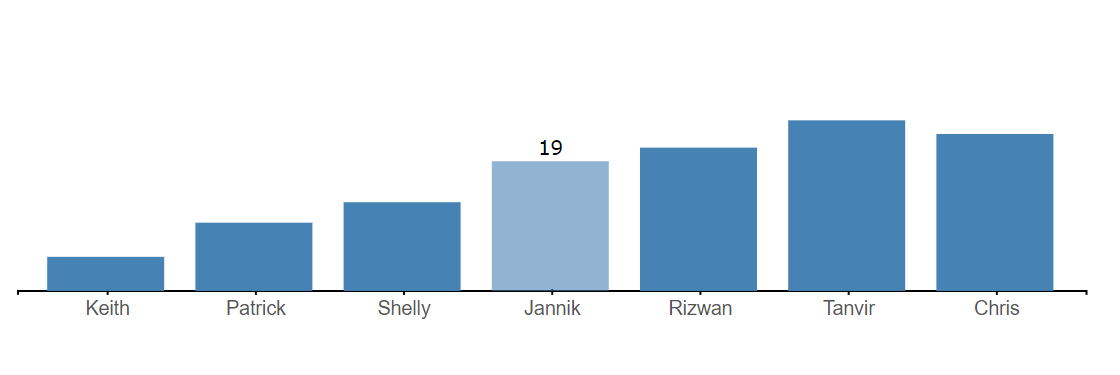
\includegraphics[width=0.47\linewidth]
{images/resp-bar-1.png}%
\label{fig:RespBarExample1}%
}
\hfill
\subfloat[][%
50rem
]
{%
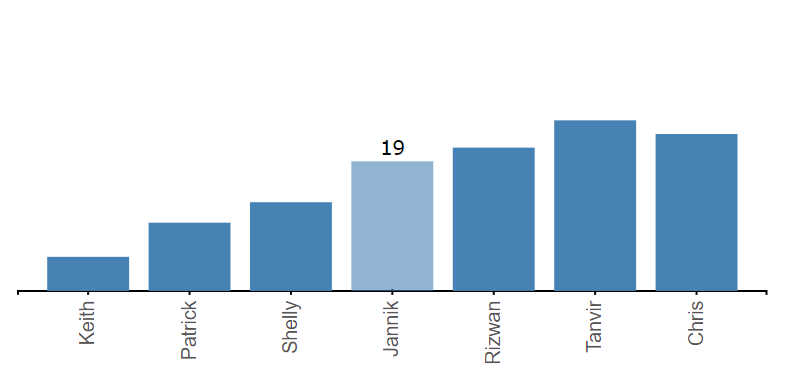
\includegraphics[width=0.33\linewidth]
{images/resp-bar-2.png}%
\label{fig:RespBarExample2}%
}
\hfill
\subfloat[][%
30rem
]
{%
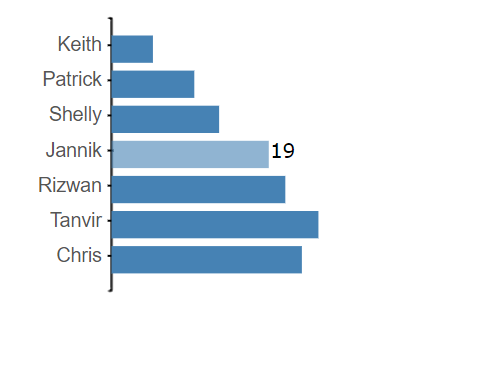
\includegraphics[width=0.2\linewidth]
{images/resp-bar-3.png}%
\label{fig:RespBarExample3}%
}
\caption[Responsive Bar Chart Example]
{
An example of a responsive bar chart at different display widths. \subref{fig:RespBarExample1} Axis tick labels are aligned horizontally. \subref{fig:RespBarExample2} Axis tick labels are aligned vertically. \subref{fig:RespBarExample3} Chart is transposed.
\imgcredit{Screenshots of \cite{RespVis} created by the author of this thesis. Used with kind permission by Keith Andrews.}
}
\label{fig:RespBarExample}
\end{figure}

The second most frequent types of responsive charts according to the responsive visualization gallery created by \cite{DesignPatternsTradeOffsRespVis} are line charts, which amount to 98 (= 26\%) out of the 378 responsive visualizations in the gallery. Line charts are used to show trends in two-dimensional datasets by plotting them as points that are then connected by lines. They can be extended to compare trends in multiple dimensions with each other by drawing additional points and lines for every additional dimension that shall be compared. Many line charts on the web are still published in non-responsive forms \parencite{HLine,HLine2}, though some web authors already took the extra effort to make their charts responsive. The minimum that can be done to make a line chart responsive is to reduce their width \parencite{RespRadialScatterHLine} by shrinking the horizontal distance between neighboring points. This usually occurs together with the recomposition and simplification of horizontal ticks. If the chart contains annotations, it may also be necessary to recompose, relocate, and simplify them as well \parencite{RespHLines,RespHLine,RespHBarHLine,RespHLineHStackedBar}. A good demonstration of which responsive patterns can be applied to make a line chart responsive is shown in the responsive line chart created by \cite{RespVis} that can be seen in Figure \ref{fig:RespLineExample}. In addition to the recomposition of ticks, tick labels are rotated to reduce their required horizontal space. For exceptionally limited space, it can make sense to remove the axes of a line chart entirely and turn it into a sparkline. However, it should be noted that by doing this, the consumer of the visualization looses a lot of information about the type and scale of the chart's dimensions. This technique should therefore only be applied in cases where no other pattern is applicable or if the trend in the data is the most important message to convey. It is rare to encounter transposed versions of line charts, though the transposing could benefit heavily annotated line charts \parencite{VLine}. Applying a transpose pattern would allow the chart to take up as much vertical space as necessary to neatly fit all the annotations without requiring the consumer to scroll horizontally.

\begin{figure}[tp]
\centering
\subfloat[][%
65rem
]
{%
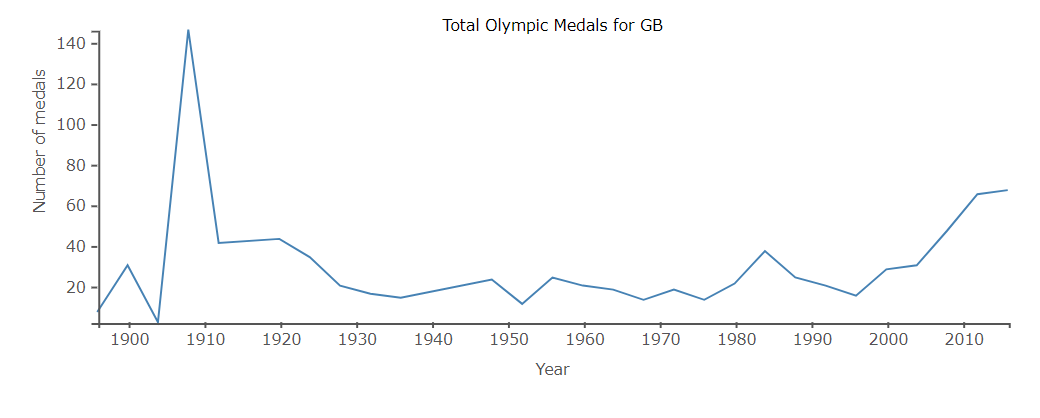
\includegraphics[width=0.52\linewidth]
{images/resp-line-1.png}%
\label{fig:RespLineExample1}%
}
\hfill
\subfloat[][%
40rem
]
{%
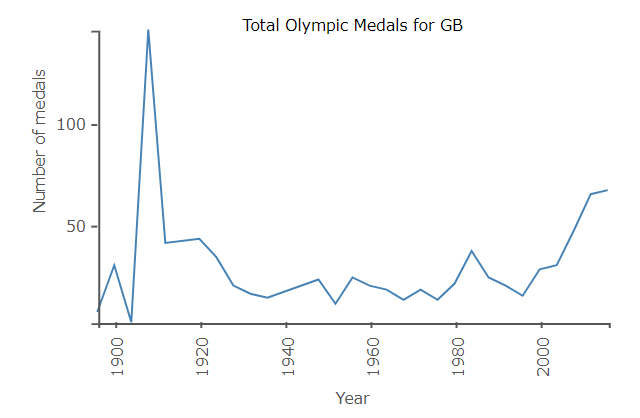
\includegraphics[width=0.31\linewidth]
{images/resp-line-2.png}%
\label{fig:RespLineExample2}%
}
\hfill
\subfloat[][%
20rem
]
{%
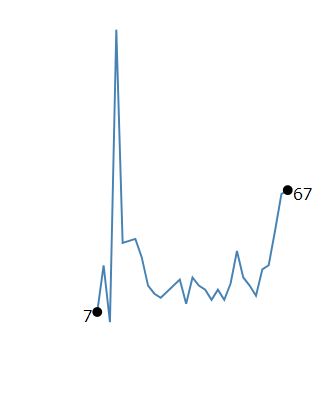
\includegraphics[width=0.16\linewidth]
{images/resp-line-3.png}%
\label{fig:RespLineExample3}%
}
\caption[Responsive Line Chart Example]
{
An example of a responsive line chart at different display widths. \subref{fig:RespLineExample1} Maximum width configuration is shown. \subref{fig:RespLineExample2} Axis ticks are thinned out and labels are rotated. \subref{fig:RespLineExample3} Axes are removed, turning the chart into a sparkline.
\imgcredit{Screenshots of \cite{RespVis} created by the author of this thesis. Used with kind permission by Keith Andrews.}
}
\label{fig:RespLineExample}
\end{figure}

Scatterplots are also among the rather frequently encountered types of responsive charts, amounting to 26 (= 7\%) of the 378 responsive charts contained in the gallery by \cite{DesignPatternsTradeOffsRespVis}. A scatterplot is a visualization that represents two-dimensional data as points in a Cartesian coordinate system. There are plenty of examples of scatterplots that are merely being published as static images \parencite{Scatter,Scatter2}, even though responsive versions can also already be observed occasionally. The first step to making scatterplots responsive is to reduce their width to fit them into the space available for them. As for other types of charts, care must be taken to avoid overlapping of labels and annotations by applying recomposition, relocation and simplification patterns \parencite{RespScatter,RespScatter2}. To counteract the increased cramming of points when reducing the size of their container, various interaction features are usually implemented in scatterplots that help consumers in making sense of the represented data. The most useful interaction features in these charts are elaborative zooming interactions and the explorative panning interactions. In addition to zooming and panning, \cite{RespVis} employs additional methods that reduce overlapping of individual points, such as fisheye distortion, Cartesian distortion or temporary displacements of points. An interesting technique for responsive visualizations that bases responsive configurations on a visualization's density rather than on its size has been introduced by \cite{NickRabinowitzRDV}. The benefit of this approach is that charts will also adapt to changing amounts of data and reconfigure their appearance accordingly. The patterns applied in the responsive scatterplot by \cite{NickRabinowitzRDV} that can be seen in Figure \ref{fig:RespScatterExample} are the recomposition of annotations to only show them for selected data records, and the switching of the encoding from a scatterplot to a heatmap for high densities. A good number of other techniques, such as for example the recomposition of data records, are also applicable to improve the responsiveness of scatterplots, but no examples for such patterns could be found. If the data that shall be encoded is inherently cyclic, a radial scatterplot, which is a polar coordinate system variant of a scatterplot, can be applied to better visualize this cyclic nature of the data \parencite{RespRadialScatterHLine}. 

\begin{figure}[tp]
\centering
\subfloat[][%
0.00005 points per pixel
]
{%
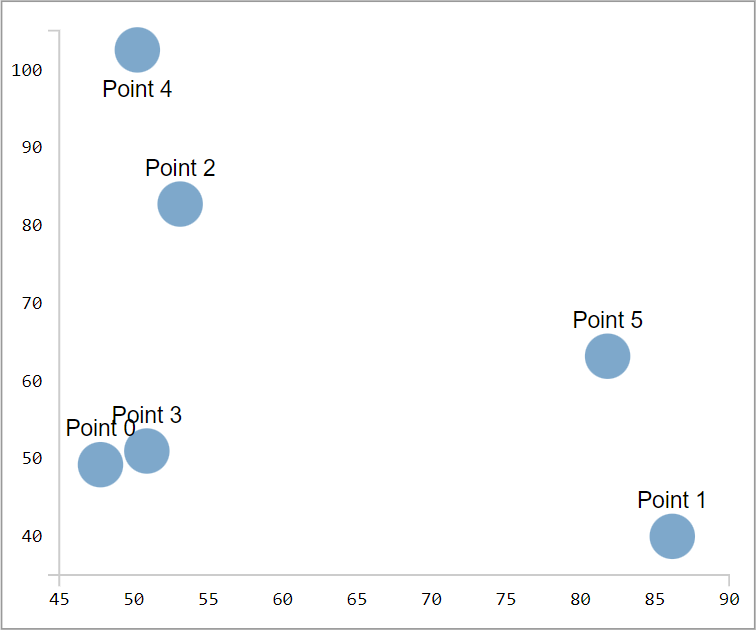
\includegraphics[width=0.33\linewidth]
{images/resp-scatter-1.png}%
\label{fig:RespScatterExample1}%
}
\hfill
\subfloat[][%
0.0007 points per pixel
]
{%
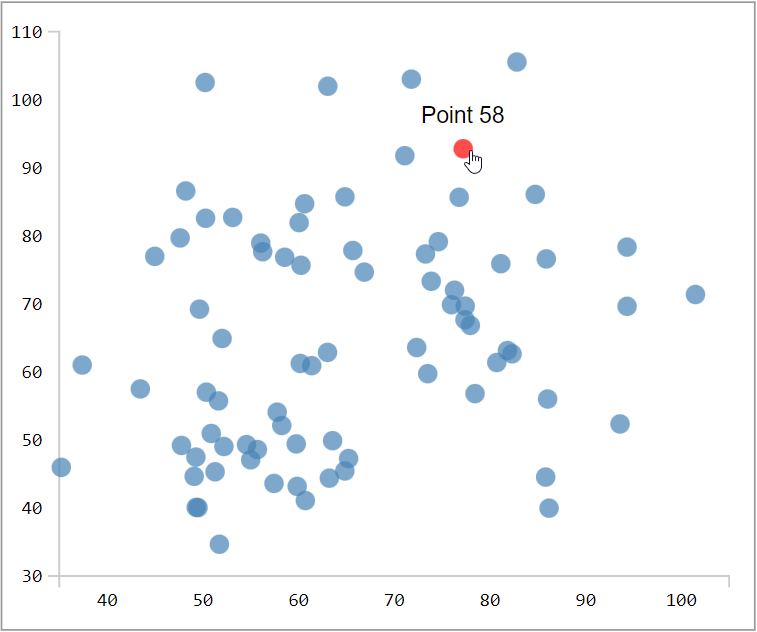
\includegraphics[width=0.33\linewidth]
{images/resp-scatter-2.png}%
\label{fig:RespScatterExample2}%
}
\hfill
\subfloat[][%
0.017 points per pixel
]
{%
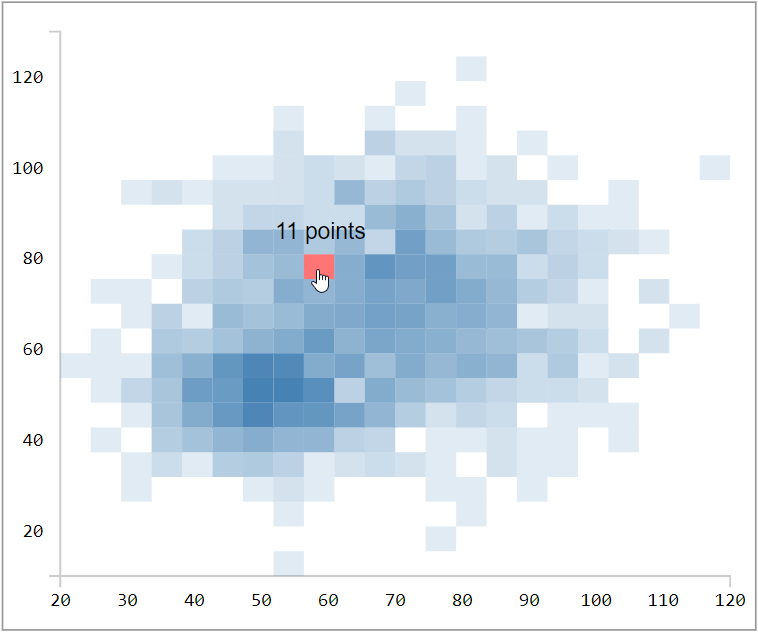
\includegraphics[width=0.33\linewidth]
{images/resp-scatter-3.png}%
\label{fig:RespScatterExample3}%
}
\caption[Responsive Scatterplot Example]
{
An example of a responsive scatterplot with increasing amount of data. The breakpoints on which the design changes are defined on the metric of data density (points per pixel) instead of on the width of the viewport as is usually the case. \subref{fig:RespScatterExample1} All points and their corresponding labels are shown. \subref{fig:RespScatterExample2} Point labels have been removed and are only shown for selected points. \subref{fig:RespScatterExample3} The scatterplot has been replaced by a heatmap to more efficiently display the large amount of data.
\imgcredit{Screenshots created by the author of this thesis. Visualization created by \cite{NickRabinowitzRDV}}
}
\label{fig:RespScatterExample}
\end{figure}

Even though parallel coordinates charts are rarely encountered in non-technical contexts, they are very popular when it comes to visualizing multidimensional data in visual analytics systems \parencite{HighD}. In these kinds of charts, multiple dimensions are rendered as parallel axes that are connected via paths. Each path represents an individual data record and its values in the corresponding dimensions. The axes of a parallel coordinates chart are typically laid out horizontally, meaning that the chart can be scaled down by reducing the distance between the individual axes. It might also be beneficial to apply previously mentioned axis-related patterns, such as rotating labels and recomposing ticks. Another technique that can be applied to make parallel coordinates charts more responsive is the successive hiding of dimensions based on their priorities. When automatically hiding dimensions, it is necessary to apply compensation patterns that give users additional controls that allow configuration of the displayed dimensions to override the system's hiding behavior. If reducing the chart's complexity is not a desirable approach, it can again be recommended to transpose the chart and expand it to whatever height necessary rather than cram too much information into the limited width available. An example of a responsive parallel coordinate chart incorporating some of these patterns can be seen in Figure \ref{fig:RespParCoordExample}.

\begin{figure}[tp]
\centering
\subfloat[][%
61rem
]
{%
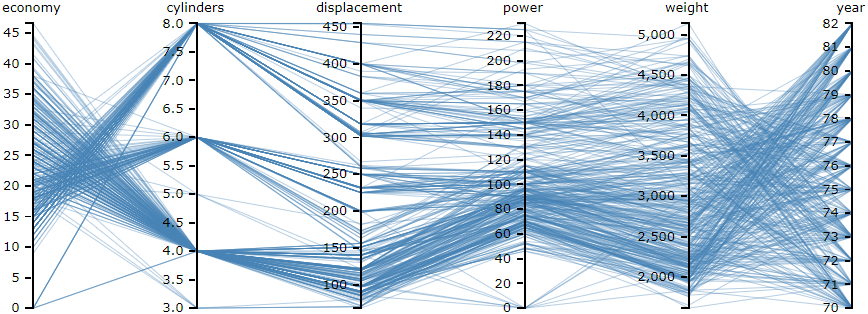
\includegraphics[width=0.55\linewidth]
{images/resp-parcoord-1.png}%
\label{fig:RespParCoordExample1}%
}
\hfill
\subfloat[][%
50rem
]
{%
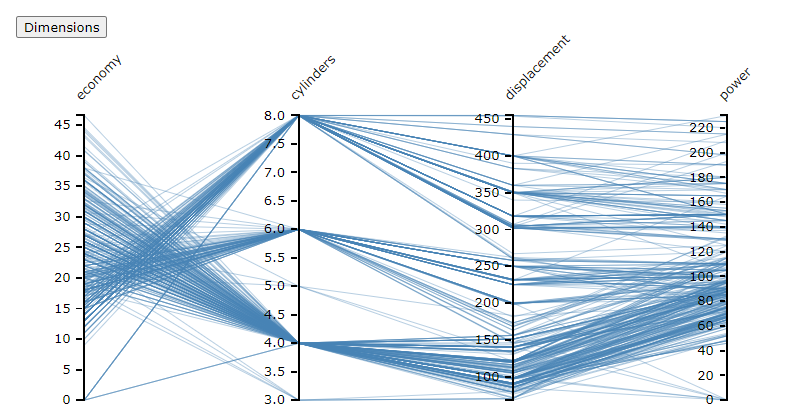
\includegraphics[width=0.45\linewidth]
{images/resp-parcoord-2.png}%
\label{fig:RespParCoordExample2}%
}
\hfill
\subfloat[][%
40rem
]
{%
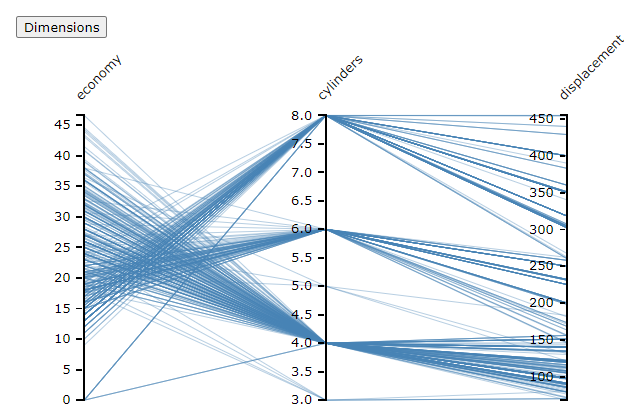
\includegraphics[width=0.4\linewidth]
{images/resp-parcoord-3.png}%
\label{fig:RespParCoordExample3}%
}
\hfill
\subfloat[][%
30rem
]
{%
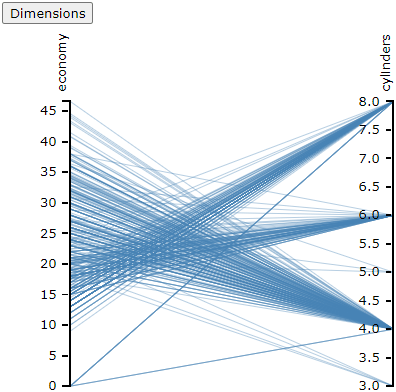
\includegraphics[width=0.3\linewidth]
{images/resp-parcoord-4.png}%
\label{fig:RespParCoordExample4}%
}
\hfill
\subfloat[][%
30rem with re-added dimensions
]
{%
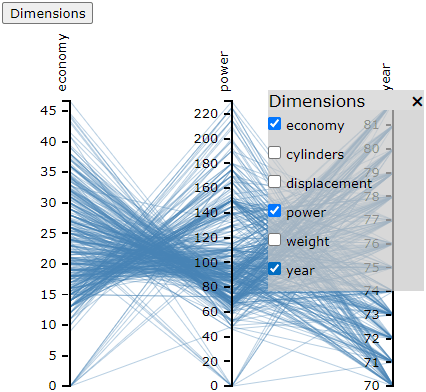
\includegraphics[width=0.3\linewidth]
{images/resp-parcoord-5.png}%
\label{fig:RespParCoordExample5}%
}
\caption[Responsive Parallel Coordinates Chart Example]
{
An example of a responsive parallel coordinates chart at different display widths. \subref{fig:RespParCoordExample1} All dimensions are shown. \subref{fig:RespParCoordExample2} Dimensions are removed based on their priority and dimension labels are rotated by 45 degrees. Also, a dimensions toggle is shown that allows configuration of dimensions. \subref{fig:RespParCoordExample3} Further dimensions are removed. \subref{fig:RespParCoordExample4} Further dimensions are removed, and dimension labels are rotated by 90 degrees. \subref{fig:RespParCoordExample5} Dimension configuration panel is opened, and a dimension has been manually re-added.
\imgcredit{Screenshots of \cite{RespVis} created by the author of this thesis. Used with kind permission by Keith Andrews.}
}
\label{fig:RespParCoordExample}
\end{figure}

% \begin{figure}[tp]
% \centering
% \subfloat[][%
% 43rem
% ]
% {%
% \includegraphics[width=0.56\linewidth]
% {images/resp-radial-scatter-1.png}%
% \label{fig:RespRadialScatterExample1}%
% }
% \hfill
% \subfloat[][%
% 34rem
% ]
% {%
% \includegraphics[width=0.44\linewidth]
% {images/resp-radial-scatter-2.png}%
% \label{fig:RespRadialScatterExample2}%
% }
% \caption[Responsive Radial Scatterplot Example]
% {
% \TODO{Maybe remove this example because of copyright?}
% . \subref{fig:RespRadialScatterExample1} . \subref{fig:RespRadialScatterExample2} . \imgcredit{Screenshots made by the author of this thesis. Visualization created by \cite{LuringMinersToTheStars}}
% }
% \label{fig:RespRadialScatterExample}
% \end{figure}

\section{Information Visualization Libraries for the Web}

For this thesis, a total of 20 JavaScript charting libraries have been collected and compared by different factors such as their rendering technology, usage popularity, open source popularity, license, and recent development activity. In terms of rendering technology, most libraries were either rendered as SVG documents or canvas elements, though some implement a hybrid renderer that could be configured to render as either one of them. Usage popularity has been measured by the cumulative package downloads from the npm package manager over the last twelve months. This has been deemed one of the most relevant metrics for the comparison because it reflects actual user behavior and gives an indication for how widespread a library is used in practice. The 22 libraries that were found in the initial collection phase were filtered by their usage popularity and recent development activity to remove those that were not sufficiently used and maintained anymore. This filtering step yielded the ten libraries that are listed in Table \ref{tab:InfoVisLibraries}. These libraries have been selected for deeper evaluation because they are heavily used and, for the most part, still actively maintained. The focus of this more detailed analysis is on summarizing the selected libraries based on high-level features and responsive capabilities. For readability reasons, the various libraries are sometimes referred to by their identifiers L1 to L10 in the following paragraphs.

Out of those ten libraries, eight are completely free to use without restrictions, amCharts has a free license for users that are comfortable with an attribution logo on their visualizations, and Highcharts offers a free license option for non-profit, educational and personal applications. Nine libraries implement a renderer that is based on SVG, two of which (ECharts, D3FC) offer alternative rendering to canvas elements for high-performance scenarios, and only Chart.js purely targets canvas-based rendering. Eight libraries are very actively maintained with most of them showing development activity in the last month. Only C3.js and Chartist seem to not be actively maintained anymore, but they nonetheless have been included in the deeper evaluation because of their historic and thematic relevance and because they are still widely used. 

In terms of APIs, visualization libraries have a strong inclination towards designing their APIs according to principles of declarative programming. APIs following these principles allow users to describe a desired state that they want the underlying system to be in. This is in strong contrast to the typical imperative way of designing APIs in which users are given a set of tools to query and modify the state of an underlying system. The difference can be summarized in simple terms as: Using declarative APIs, users specify what state shall be achieved, whereas when using imperative APIs, users specify how a certain state is achieved. Declarative APIs are usually built on top of lower-level imperative APIs and can therefore be seen as a higher level of abstraction over them. They are popular among developers because they are expressive, easy to use and effectively encapsulate complexity that would otherwise have to be handled by users. An often overlooked disadvantage of declarative APIs is that they frequently only provide high-level access to a system and that more specific use cases might not be achievable if they can not be expressed in the domain specific language (DSL) defined by the API. In many cases it makes sense to provide additional optional imperative APIs for users that require a lower level of access to the system to enable them to implement functionality not covered by the declarative parts of the interface.

All evaluated libraries, except D3FC, expose declarative interfaces in the form of nested configuration objects used to specify the characteristics of individual visualizations. Apart from Chartist, all those libraries feature generic high-level functions that create charts from declarative configuration objects that allow the specification of different forms of visualization for different data dimensions. These generic chart creation functions seem to be correlated with the ability of dynamically changing the type of visualization. In Chartist, for instance, which provides separate chart creation functions for each type of chart, it is not possible to alter the type of chart after it has been created. Another limitation that may originate in this interface partitioning via chart types is that mixed charts that combine multiple forms of visualization in one composite visualization can not be expressed. The only library in the deeper evaluation that does not provide a high-level declarative configuration API is D3FC. The design philosophy of D3FC is based on the idea of "unboxing" D3, which is a powerful, low-level library for data-driven rendering of documents \parencite{D3}. Many visualization libraries are implemented with D3, but it is usually hidden behind public APIs that are easier to work with but which don't provide the full flexibility that D3 does. D3FC exposes a component-based interface that closely follows design patterns commonly encountered in various D3 modules. These components form higher-level building blocks on which advanced visualizations can be built. They are also highly configurable and in those cases where the options for configuration are not sufficient, a decorator pattern is used to allow users to hook into the underlying D3 functionality and inject custom code into the various stages of the general update pattern at the core of D3. 
amCharts
hybrid API
generic declarative configuration API
component-based API similar to D3FC
users can use whichever they prefer 

\subsection{Data-Driven Documents (D3)}

D3 \parencite{D3} is a free and open-source document manipulation library built in JavaScript. It is maintained by an active GitHub community and its core maintainer Mike Bostock who is also the creator of Observable \parencite{Observable} and the deprecated Protovis library \parencite{Protovis}. 

D3 enables data-driven document transformations that allow developers to describe their documents as functions of data. As an example, developers can define transformations that receive a dataset and transform it into a basic HTML table or into a more sophisticated visualization as an SVG chart. This focus on explicitly defining transformations is better suited for dynamic visualizations because developers have complete control over the creation, modification and removal of elements. It also sets D3 apart from other visualization libraries where developers usually define the desired state of a representation using a declarative domain specific language.

In contrast to other visualization libraries, D3 contains no proprietary visual primitives and relies on well established web standards like HTML, SVG and CSS to provide visual representations. This yields a lot of flexibility because developers work directly with web standards that are implemented by their browsers and do not need to wait for D3 to implement support for new features as standards evolve. If developers chose to switch to a different library, the knowledge of web standards they gained during their work with D3 might be applicable in their future work. The reliance on web standards also makes it possible to use debugging tools that are already natively implemented in browsers.

Other important aspects of D3's design include immediate evaluation, the principle of parsimony, and support for method chaining. Immediately evaluating functions means that operations, such as modifying attributes, are applied instantaneously at the time of calling the respective functions. This achieves a reduction in internal complexity by handing it over to invoking code and avoids common errors related to missing state changes when state is being modified multiple times between rendering. The principle of parsimony, also referred to as Occam's razor, is a problem-solving principle that stems from the field of philosophy \parencite{PrincipleOfParsimony}. It is frequently paraphrased as "entities should not be multiplied beyond necessity" and when applied to API design it means that superfluous functions in an API should be avoided. As an example, the background color of a circle element can already be set with the generic \lstinline{Selection.attr} method to set the \attrname{background-color} attribute of all elements in a Selection. Adding an additional \lstinline{backgroundColor} method would violate the principle of parsimony. Method chaining is a popular syntax that allows functions to be chained after one another to avoid having to store intermediate results into variables that would otherwise not be needed. It is implemented in D3 by returning the \lstinline{Selection} on which a modifying method is called as a result of that method. Methods that insert new elements into the DOM, such as \lstinline{Selection.append} and \lstinline{Selection.insert}, return a Selection of the newly added elements instead to enable the creation of nested structures. This method chaining syntax is further improved by the \lstinline{Selection.call} method that invokes a callback receiving the current Selection as a parameter and returns the original Selection to further chain methods on it after the callback has been executed. The \lstinline{Selection.call} method enables the creation of complex method chaining structures and is widely used by developers. A simple example of method chaining in D3 and the application of the \lstinline{Selection.call} method can be seen in Figure \ref{list:D3MethodChaining}.

\begin{samepage}
\lstinputlisting[%
  float=tp,
  aboveskip=\floatsep,
  belowskip=\floatsep,
  xleftmargin=0cm,              % no extra margins for floats
  xrightmargin=0cm,             % no extra margins for floats
  %
  language=JavaScript,
  basicstyle=\footnotesize\ttfamily,
  frame=shadowbox,
  numbers=left,
  label=list:D3MethodChaining,
  caption={
    [D3 Method Chaining] A simple example of method chaining in D3 that creates an \tagname{h1} and \tagname{p} element inside a \tagname{body}.
  },
]{listings/d3-method-chaining.js}
\end{samepage}

Selections have already been mentioned in the previous paragraphs. They are the atomic building blocks of D3 that are used to access almost any functionality. Selections are created using the \lstinline{d3.select} or \lstinline{d3.selectAll} methods. These methods are built on the DOM Selectors API, namely the \lstinline{querySelector} and \lstinline{querySelectorAll} methods, which allow the selection of elements via CSS selectors (see Section \ref{sec:CSS}), and which consequentially allow the \lstinline{d3.select} and \lstinline{d3.selectAll} methods to either create a Selection containing a single element matching the provided selector or to create one that contains multiple elements matching it. A Selection acts as a wrapper container around these selected elements, and it provides methods to perform frequently performed DOM operations on them. Among others, the element operations provided by a Selection include the setting and getting of: Attributes using the \lstinline{Selection.attr} method, styles using the \lstinline{Selection.style} method, properties using the \lstinline{Selection.property} method, text or HTML content using the \lstinline{Selection.text} or \lstinline{Selection.html} methods, and event listeners using the \lstinline{Selection.on} method. Selections also provide wrapper methods to add additional elements to the document using the \lstinline{Selection.append} or \lstinline{Selection.insert} methods as well as to remove them using the \lstinline{Selection.remove} method. Accessing the DOM using these methods is less tedious because the API that is natively provided by the DOM is very verbose and also because the method chaining API provided by D3 does not require intermediate variables where none are needed.

An additional feature that D3 adds is the ability to bind data to elements using the \lstinline{Selection.data} and \lstinline{Selection.datum} methods. The \lstinline{Selection.datum} method binds a single provided data record to all elements in the Selection, whereas the \lstinline{Selection.data} method receives an array of data records and binds each individual data record to exactly one element. The \lstinline{Selection.data} method performs a join operation between data and elements to ensure that exactly one element per data record exists. This data join results in three separate Selections: the enter Selection, containing the elements that were newly created, the update Selection, containing the elements that merely receive new data, and the exit Selection, containing the elements that are being removed. Each of these Selections can be individually transformed using the \lstinline{Selection.join} method, which can receive three callbacks each being respectively invoked with the enter, update and exit Selections of the data join. This ability of individually controlling updates of entering, updating and exiting elements is being referred to as the general update pattern in D3 and a simple demonstration of how it is used can be seen in Figure \ref{list:D3GeneralUpdatePattern}. All the previously mentioned DOM wrapper methods can receive either constant values or dynamic ones that are defined as functions. These functions receive the bound element data, the element's index in the group of nodes represented by the Selection, and the group of nodes themselves as input and calculate a dynamic value based on these parameters, which is then forwarded to the corresponding DOM methods. 

\begin{samepage}
\lstinputlisting[%
  float=tp,
  aboveskip=\floatsep,
  belowskip=\floatsep,
  xleftmargin=0cm,              % no extra margins for floats
  xrightmargin=0cm,             % no extra margins for floats
  %
  language=JavaScript,
  basicstyle=\footnotesize\ttfamily,
  frame=shadowbox,
  numbers=left,
  label=list:D3GeneralUpdatePattern,
  caption={
    [D3 General Update Pattern] A demonstration of D3's general update pattern and how it can be used to specify different transformations for entering, updating and exiting elements.
  },
]{listings/d3-join.js}
\end{samepage}

D3 also offers a convenient and optional API to perform JavaScript-based animations via Transitions, which wrap a Selection and allow the animation of various element characteristics. Transitions are created using the \lstinline{Selection.transition} method that creates a Transition wrapping the  Selection on which it has been called. The duration of a Transition is defined using the \lstinline{Transition.duration} method, it's easing can be configured using the \lstinline{Transition.ease} method, and there is also the possibility of interrupting and chaining transitions, but explaining these things would be to go into too many details. Transitions provide an (almost) identical API to Selections. The major change is that the wrapping methods interpolate towards their target values using the set easing function over the set duration instead of setting the target value directly. Using D3 Transitions is completely optional and users can also choose to use other animation technologies, like CSS transitions and animations, instead.

At the core, D3 is simply a low-level library to perform data-driven document transformations. Even though this generic core technology is applicable to a wide range of use cases, D3 has been created with a focus on creating visualizations. Many additional modules exist that simplify performing the higher-level tasks necessary for the rendering of visualizations and despite these functionalities being split on multiple modules, they all follow the same patterns inherent to D3 like method chaining. Most modules are implemented as configurable functions that are configured using chainable functions and which can be invoked after configuration to perform a specific action. Listing all available modules here would be out of the scope of this work but some noteworthy and characteristic ones include: \modname{d3-shape} to create visual primitives like lines and areas, \modname{d3-scale} to encode abstract data dimensions, \modname{d3-axis} to render scales as human-readable axes, and many more such as \modname{d3-array}, \modname{d3-layout} and \modname{d3-zoom}. 


% D3
% https://ieeexplore.ieee.org/abstract/document/6064996?casa_token=qjwRCVBvvlwAAAAA:aE54yNnqeUkw7U-Zaab-4Idn00G4kTfXi1b_LT40Eka6PBbzxmKPpodvJWSUn2TzjdQtWFFMtYwJ

% Protovis
% https://ieeexplore.ieee.org/abstract/document/5290720?casa_token=gLceJJ7RJnAAAAAA:ufCN6a1-ydmZFR7Y9yFyLRkYpvJlzo5ZihfcR1myK6-UEfpyWlQNr6knb_FrBpdfXC8eaXmEgp8r

% PrincipleOfParsimony
% https://www.journals.uchicago.edu/doi/abs/10.1093/bjps/32.2.145?journalCode=bjps

% A lot of libraries exist that simplify the creation of of visualizations on the web. On the first glance, most of those libraries seem interchangeable because their interfaces are very similar. In many cases there is a generic high-level creation function that is invoked with a nested options object specifying the type of chart that shall be generated and its configuration. Some libraries separate their interface by chart types, which usually leads to the limitation that the type of an already created visualization can not be changed dynamically. 


% Most libraries offer special chart types that are used to combine other types of charts into composite visualizations.